\documentclass[11pt]{article}
\usepackage[paperwidth=16cm,paperheight=9cm,margin=0.7cm,top=0.6cm,bottom=0.5cm]{geometry}
\usepackage[T1]{fontenc}
\usepackage[scaled=0.95]{helvet}\renewcommand{\familydefault}{\sfdefault}
\usepackage{amsmath,amssymb}
\usepackage{graphicx,xcolor,booktabs,enumitem,tikz}
\usetikzlibrary{arrows.meta,positioning}
\usepackage[hidelinks]{hyperref}
\graphicspath{{../figures/}}
\pagestyle{empty}
\setlength{\parindent}{0pt}
\definecolor{acc}{HTML}{1F3A5F}
\definecolor{acc2}{HTML}{C0392B}
\setlist{itemsep=3pt,topsep=3pt,leftmargin=1.2em}
\newcommand{\slide}[1]{\newpage\raggedright{\color{acc}\Large\bfseries #1\par}\vspace{1pt}{\color{acc}\rule{\linewidth}{0.8pt}}\par\vspace{5pt}}
\newcommand{\Ot}{\tilde O}

\begin{document}
\small\raggedright

% ---------------------------------------------------------------- title
\thispagestyle{empty}
\vspace*{0.5cm}
{\color{acc}\LARGE\bfseries Breaking the Bellman--Ford Barrier\par}
\vspace{4pt}
{\large Efficient Shortest-Path Algorithms for Graphs with Negative Edge Weights\par}
\vspace{6pt}
{\color{acc}\rule{\linewidth}{1pt}}
\vspace{6pt}

CSD319 Design and Analysis of Algorithms: End-Term Project (Problem 2)\par
Shiv Nadar Institution of Eminence, November 2026
\vfill
\begin{tabular}{@{}ll@{\hspace{1.5cm}}ll@{}}
Pragun Kathuria & 2410110237 & Tanvi Pandey & 2410110356\\
Amitoj Oberoi & 2410110046 & Vishnu Sriram & 2410110629\\
\end{tabular}

% ---------------------------------------------------------------- problem
\slide{Problem Statement}
\begin{minipage}[t]{0.58\linewidth}
\textbf{Input:} directed $G=(V,E)$, $n$ vertices, $m$ edges, weights $w:E\to\mathbb R$ (may be negative), source $s$.

\medskip
\textbf{Output:} either
\begin{itemize}
\item $\delta(s,v)$ for all $v$ plus a shortest-path tree, or
\item a \textbf{negative cycle certificate} reachable from $s$.
\end{itemize}

\medskip
\textbf{Why it matters:} arbitrage detection, difference constraints (scheduling), min-cost flow, Johnson's APSP.
\end{minipage}\hfill
\begin{minipage}[t]{0.38\linewidth}
\textbf{Dijkstra fails:}\par\medskip
\centering
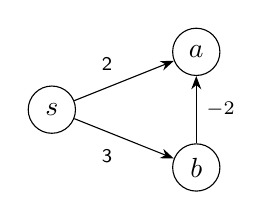
\begin{tikzpicture}[>=Stealth, every node/.style={circle,draw,minimum size=6mm,inner sep=0}]
\node (s) {$s$};
\node (a) [above right=0.3cm and 1.4cm of s] {$a$};
\node (b) [below right=0.3cm and 1.4cm of s] {$b$};
\draw[->] (s) -- node[draw=none,above left]{\scriptsize 2} (a);
\draw[->] (s) -- node[draw=none,below left]{\scriptsize 3} (b);
\draw[->] (b) -- node[draw=none,right]{\scriptsize $-2$} (a);
\end{tikzpicture}\par\smallskip
\raggedright\footnotesize Dijkstra fixes $\delta(a)=2$; truth is $1$.\\
For 60+ years, the best general bound was Bellman--Ford's $O(nm)$.
\end{minipage}

% ---------------------------------------------------------------- algorithms
\slide{Algorithms Studied}
\begin{minipage}[t]{0.49\linewidth}
\textbf{Classical / practical (implemented)}
\begin{itemize}
\item \textbf{Bellman--Ford}: $n-1$ passes over all edges
\item \textbf{Early termination}: stop when a pass changes nothing
\item \textbf{Yen}: forward/backward DAG passes, $\le\lceil n/2\rceil$ passes
\item \textbf{Randomized Yen} (Bannister--Eppstein): $\approx nm/3$ expected
\item \textbf{SPFA}: queue of ``active'' vertices
\item \textbf{Johnson}: reweighting $\Rightarrow$ $n\times$ Dijkstra for APSP
\item \textbf{Hybrid (ours)}
\end{itemize}
\end{minipage}\hfill
\begin{minipage}[t]{0.47\linewidth}
\textbf{Theoretical breakthroughs (surveyed)}
\begin{itemize}
\item Goldberg 1995: $O(\sqrt n\,m\log W)$ (scaling)
\item Bernstein--Nanongkai--Wulff-Nilsen 2022: $O(m\log^8 n\log W)$, FOCS best paper
\item Bringmann--Cassis--Fischer 2023: $O(m\log^2 n\log(nW)\log\log n)$
\item Fineman 2024: $\Ot(mn^{8/9})$ for \emph{real} weights
\item Huang--Jin--Quanrud 2025: $\Ot(mn^{4/5})$
\end{itemize}
\end{minipage}

% ---------------------------------------------------------------- key idea
\slide{Key Tool: Certificates from the Predecessor Graph}
\begin{itemize}
\item Each vertex keeps $\pi(v)$ = last vertex that improved it. The graph $G_\pi$ has in-degree $\le 1$, so a cycle search costs $O(n)$.
\item \textbf{Lemma.} Every cycle in $G_\pi$ is a negative cycle of $G$.\\[2pt]
{\footnotesize\emph{Proof idea:} each pointer edge satisfies $d(v)\ge d(u)+w(u,v)$. The relaxation that closes the cycle is strict. Summing around the cycle, the labels cancel and $0>w(C)$.}
\item Checking $G_\pi$ once per pass (or every $n$ updates) costs $O(1)$ amortized per relaxation.
\item Certificates are \textbf{verifiable}: no false positives, and detection comes long before Bellman--Ford's $n$-th pass.
\end{itemize}

% ---------------------------------------------------------------- hybrid
\slide{Our Hybrid Variant}
\begin{minipage}[t]{0.55\linewidth}
\begin{enumerate}
\item \textbf{Yen passes with a BFS ranking} from $s$ ($O(n+m)$ preprocessing): most shortest-path edges become ``forward'', so long runs are fixed in one half-pass.
\item \textbf{Early termination} when a pass changes nothing.
\item \textbf{$G_\pi$ cycle check after every pass}, giving an early certificate.
\end{enumerate}
\end{minipage}\hfill
\begin{minipage}[t]{0.41\linewidth}
\textbf{Guarantees}
\begin{itemize}
\item Yen's theorem holds for \emph{any} ranking, so at most $\lceil n/2\rceil+1$ passes
\item Worst case $O(nm)$, about half of Bellman--Ford
\item Certificates are correct by the lemma
\end{itemize}
\end{minipage}

% ---------------------------------------------------------------- proofs
\slide{Proof of Correctness: Main Results}
\begin{itemize}
\item \textbf{Upper bound:} $d(v)\ge\delta(v)$ always, and finite labels are weights of real walks.
\item \textbf{Path relaxation:} relaxing the edges of a shortest path in order makes its endpoint correct.
\item \textbf{Bellman--Ford:} shortest paths have $\le n-1$ edges, and pass $i$ fixes edge $i$.
\item \textbf{Detection:} if a reachable cycle $C$ has $w(C)<0$, summing the triangle inequalities gives $0\le w(C)$, a contradiction. So some edge is always still relaxable.
\item \textbf{Yen:} a path splits into $r\le n-1$ alternating monotone runs. Each half-pass fixes a whole run (a DAG in topological order), so $\lceil n/2\rceil$ passes suffice.
\item \textbf{SPFA:} each vertex appears in at most one queue round, and there are $\le n-1$ rounds, so $n$ dequeues certify a cycle.
\item \textbf{Johnson:} $\hat w(u,v)=w(u,v)+h(u)-h(v)\ge0$ telescopes along paths, so shortest paths are preserved.
\end{itemize}

% ---------------------------------------------------------------- complexity
\slide{Complexity Analysis}
\centering\footnotesize
\begin{tabular}{@{}llll@{}}
\toprule
\textbf{Algorithm} & \textbf{Worst-case time} & \textbf{Weights} & \textbf{Type}\\
\midrule
Bellman--Ford & $\Theta(nm)$ & real & det.\\
+ early stop & $O(hm)$ if no neg.\ cycle ($h$ = hop depth) & real & det.\\
Yen / Hybrid & $\approx nm/2$ & real & det.\\
Randomized Yen & $\approx nm/3$ expected & real & rand.\\
SPFA & $O(nm)$ & real & det.\\
Johnson (APSP) & $O(nm+n^2\log n)$ & real & det.\\
Floyd--Warshall (APSP) & $\Theta(n^3)$ & real & det.\\
\midrule
Goldberg 1995 & $O(\sqrt n\,m\log W)$ & integer & det.\\
BNW 2022 / BCF 2023 & $O(m\log^8 n\log W)$ / $O(m\log^2 n\log(nW)\log\log n)$ & integer & rand.\\
Fineman 2024 / HJQ 2025 & $\Ot(mn^{8/9})$ / $\Ot(mn^{4/5})$ & real & rand.\\
\bottomrule
\end{tabular}

% ---------------------------------------------------------------- experiments 1
\slide{Experiments: No Negative Cycle}
\begin{minipage}{0.49\linewidth}
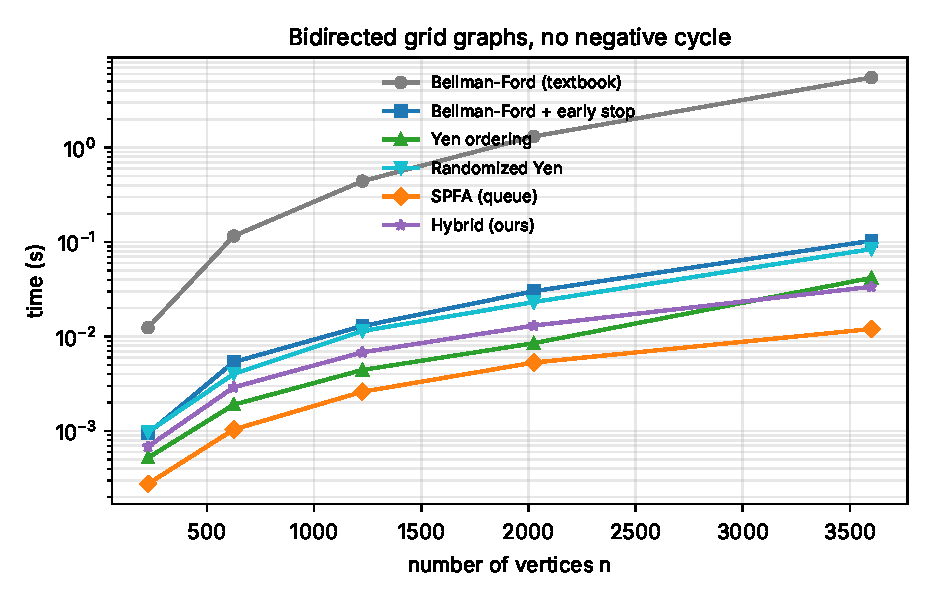
\includegraphics[width=\linewidth]{grid_time.pdf}
\end{minipage}\hfill
\begin{minipage}{0.49\linewidth}
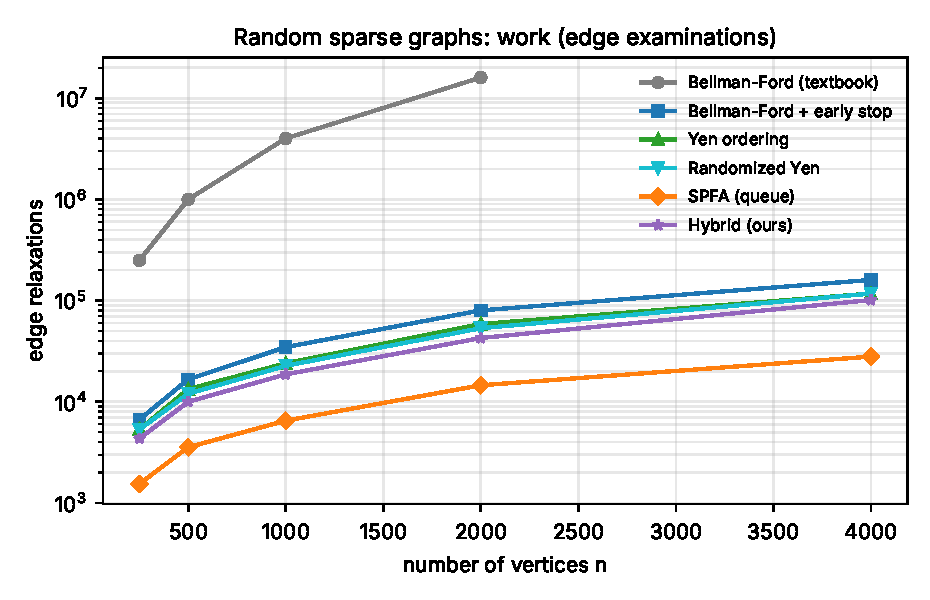
\includegraphics[width=\linewidth]{random_relax.pdf}
\end{minipage}\par\smallskip
\footnotesize Early stop cuts Bellman--Ford's work by about $200\times$ on random graphs. On grids the BFS-ordered hybrid needs about 11 passes vs.\ 64 for early-stop BF ($3\times$ faster). SPFA is the fastest when no negative cycle exists. Limitation: on an adversarial chain the BFS order does not follow the tree, and the hybrid behaves like randomized Yen ($\approx n/3$ passes, as theory predicts).

% ---------------------------------------------------------------- experiments 2
\slide{Experiments: Negative-Cycle Detection}
\begin{minipage}{0.49\linewidth}
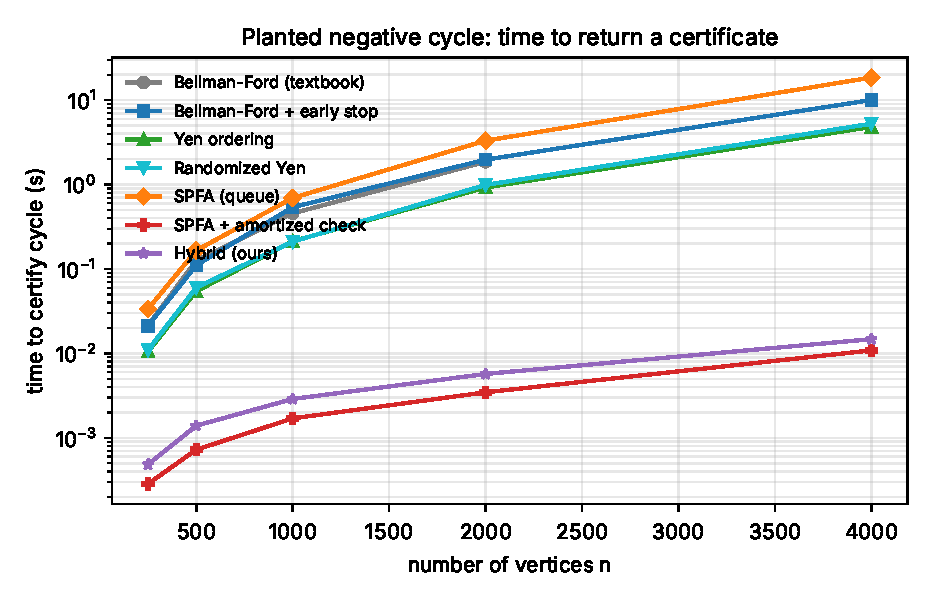
\includegraphics[width=\linewidth]{negcycle_time.pdf}
\end{minipage}\hfill
\begin{minipage}{0.49\linewidth}
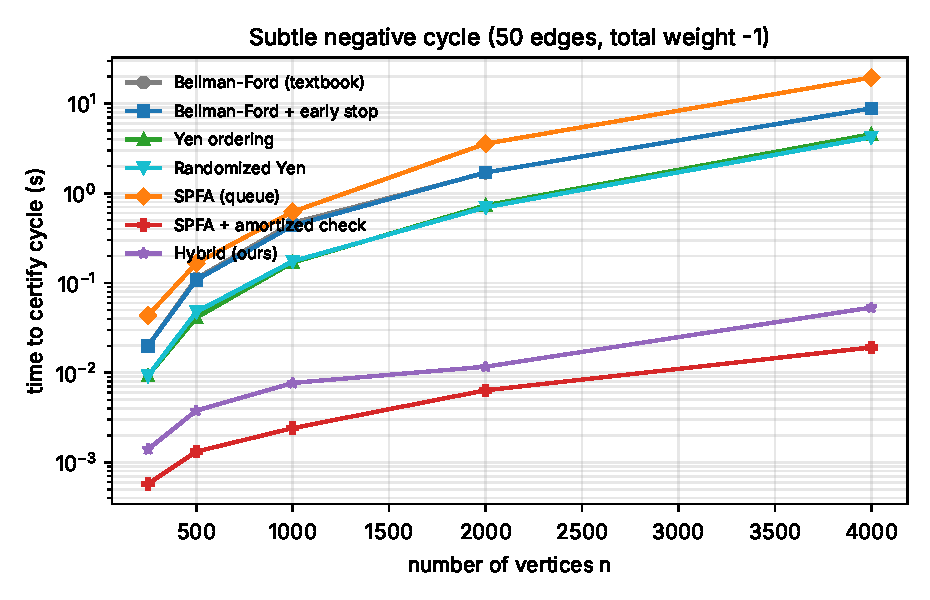
\includegraphics[width=\linewidth]{subtle_time.pdf}
\end{minipage}\par\smallskip
\footnotesize With a negative cycle, early stop never fires: BF pays all $n$ passes (10\,s at $n=4000$) and classic SPFA is even slower (18.5\,s). Predecessor-graph certificates return a verified cycle in milliseconds: the hybrid is $167$--$670\times$ faster and SPFA + amortized check about $460\times$ faster on the subtle cycle.

% ---------------------------------------------------------------- conclusion
\slide{Conclusion}
\begin{itemize}
\item All classical label-correcting methods are $O(nm)$. Orderings only improve the constant (Yen $\tfrac12$, random $\tfrac13$).
\item In practice, $nm$ is paid mainly \textbf{when a negative cycle exists}, which is exactly when classical detection is slowest.
\item \textbf{Predecessor-graph certificates} (proved always negative, $O(1)$ amortized) cut detection from seconds to milliseconds with no false positives.
\item Our \textbf{hybrid} keeps Yen's $\lceil n/2\rceil+1$ bound, is $3\times$ faster on grids and $167$--$670\times$ faster at detecting cycles, but depends on the BFS order matching the tree.
\item Beating $O(nm)$ asymptotically needs new ideas: scaling, low-diameter decompositions and randomization. Their practical value is still open.
\end{itemize}
\medskip
\textbf{Johnson vs.\ Floyd--Warshall:} $6.3\times$ faster at $n=300$ on sparse graphs.

% ---------------------------------------------------------------- gaps
\slide{Gaps and Future Directions}
\begin{itemize}
\item \textbf{Deterministic near-linear SSSP}: all $\Ot(m)$ algorithms are randomized. Deterministic $m^{1+o(1)}$ bounds need heavy min-cost-flow machinery.
\item \textbf{Real weights}: best known is $\Ot(mn^{4/5})$. Is $\Ot(m)$ possible? No lower bound is known.
\item \textbf{Shaving logs}: close the gap between BCF and $O(m\log W)$.
\item \textbf{Practicality}: engineer the near-linear algorithms and benchmark them against tuned label-correcting methods.
\item \textbf{Adaptive orderings}: re-rank vertices by the current tree while keeping worst-case and randomized guarantees.
\item \textbf{Dynamic, parallel and distributed} negative-weight SSSP.
\end{itemize}
\vfill
\centering{\color{acc}\large\bfseries Thank you! Questions?}

\end{document}
